\documentclass[a4paper,12pt,oneside]{book}

%-------------------------------Start of the Preable------------------------------------------------
\usepackage[english]{babel}
\usepackage{blindtext}
%packagr for hyperlinks
\usepackage{hyperref}
\hypersetup{
	colorlinks=true,
	linkcolor=blue,
	filecolor=magenta,      
	urlcolor=cyan,
}

\urlstyle{same}
%use of package fancy header
\usepackage{fancyhdr}
\setlength\headheight{26pt}
\fancyhf{}
%\rhead{\includegraphics[width=1cm]{logo}}
\lhead{\rightmark}
\rhead{\includegraphics[width=1cm]{logo}}
\fancyfoot[RE, RO]{\thepage}
\fancyfoot[CE, CO]{\href{http://www.e-yantra.org}{www.e-yantra.org}}

\pagestyle{fancy}

%use of package for section title formatting
\usepackage{titlesec}
\titleformat{\chapter}
{\Large\bfseries} % format
{}                % label
{0pt}             % sep
{\huge}           % before-code

%use of package tcolorbox for colorful textbox
\usepackage[most]{tcolorbox}
\tcbset{colback=cyan!5!white,colframe=cyan!75!black,halign title = flush center}

\newtcolorbox{mybox}[1]{colback=cyan!5!white,
	colframe=cyan!75!black,fonttitle=\bfseries,
	title=\textbf{\Large{#1}}}

%use of package marginnote for notes in margin
\usepackage{marginnote}

%use of packgage watermark for pages
%\usepackage{draftwatermark}
%\SetWatermarkText{\includegraphics{logo}}
\usepackage[scale=2,opacity=0.1,angle=0]{background}
\backgroundsetup{
	contents={\includegraphics{logo}}
}

%use of newcommand for keywords color
\usepackage{xcolor}
\newcommand{\keyword}[1]{\textcolor{red}{\textbf{#1}}}

%package for inserting pictures
\usepackage{graphicx}

%package for highlighting
\usepackage{color,soul}

%new command for table
\newcommand{\head}[1]{\textnormal{\textbf{#1}}}

\usepackage[export]{adjustbox}

%----------------------End of the Preamble---------------------------------------

\begin{document}

%---------------------Title Page------------------------------------------------
\begin{titlepage}
	\raggedright
	{\Large eYSIP2017\\[1cm]}
	{\Huge\scshape\centering Distributed robotics - multi swarm robots \\[.1in]}
	\vfill
		\hfill\\
	\begin{figure}[h!]
		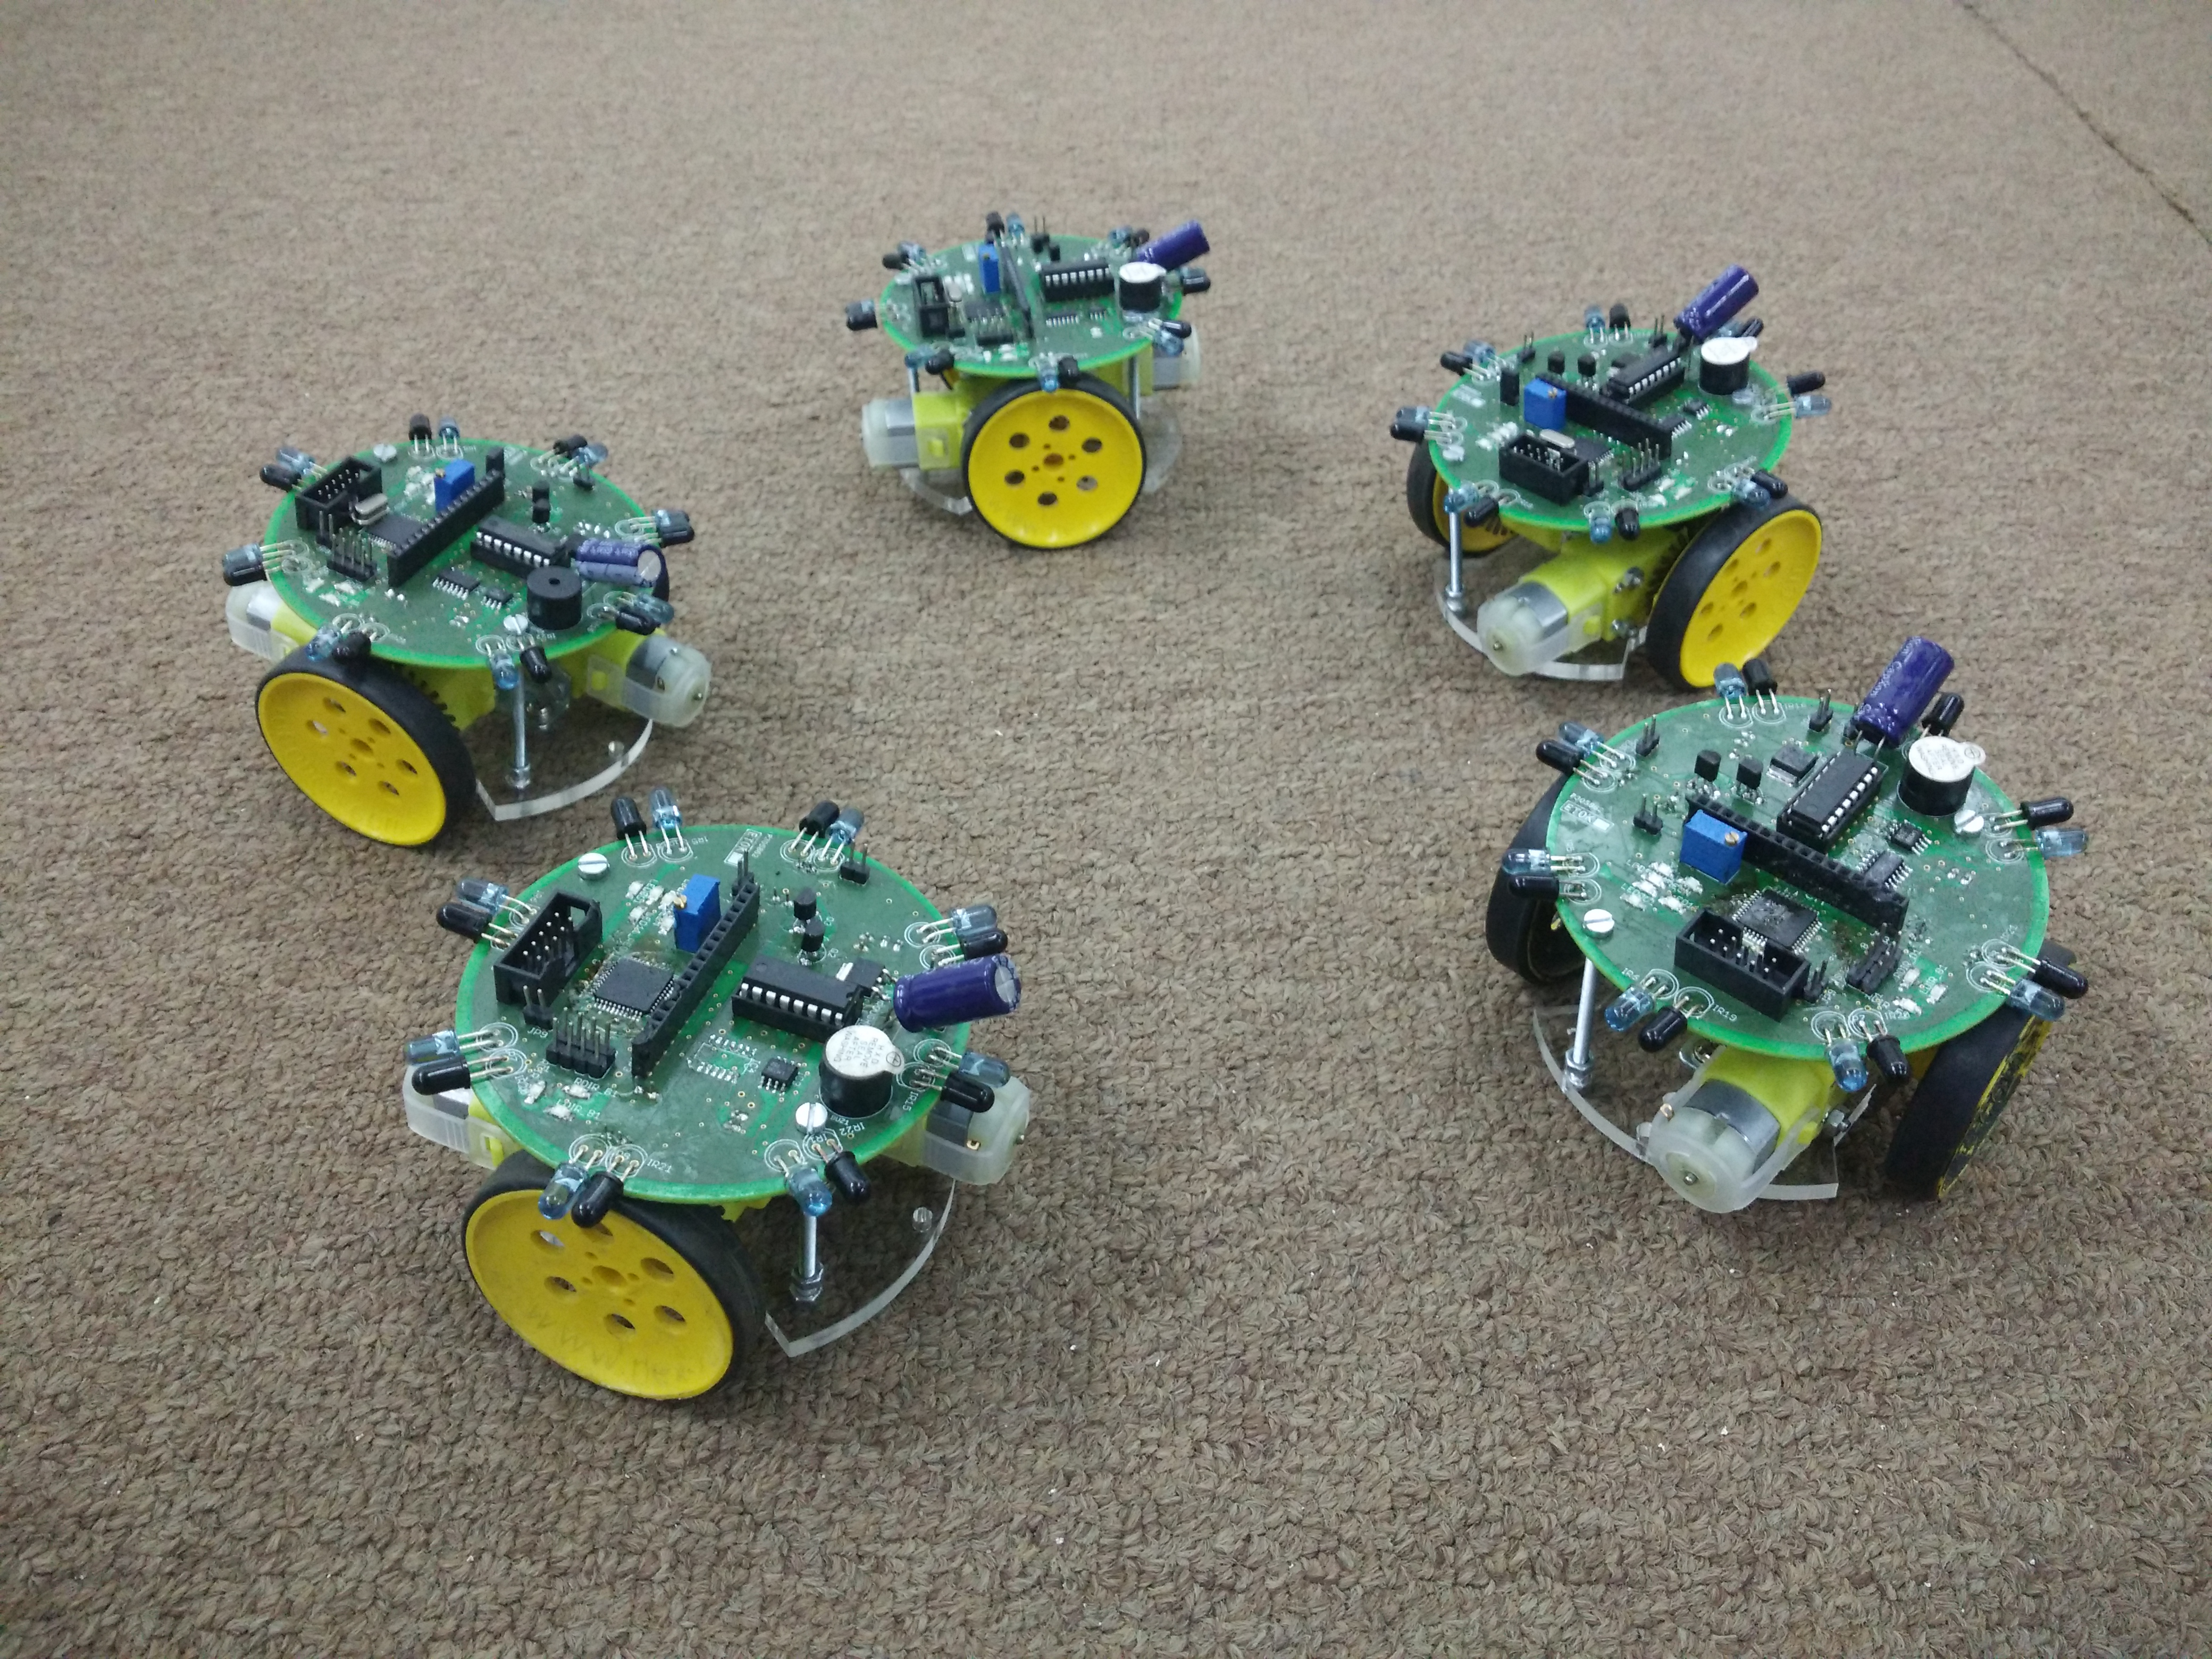
\includegraphics[width=\textwidth]{./HardwareManual/Small_bots.jpg}		
	\end{figure}	
	\hfill\\
	\begin{flushright}
		{\large Intern 1 Mr. Chinmay C \\}
		{\large Intern 2 Mr. R Hariharan \\}
		{\large Mentor 1 Ms. Rutuja \\}
		{\large Mentor 2 Ms. Deepa \\}
		{\large Duration of Internship: $ 22/05/2017-07/07/2017 $ \\}
	\end{flushright}
	
	{\itshape 2017, e-Yantra Publication}
\end{titlepage}
	
\tableofcontents

	\chapter{Introduction}
	Thanks for choosing the Mini bots mobile robot platform. Mini bots will give you good
	exposure to the world of swarm robotics and embedded systems. Thanks to its innovative architecture
	and adoption of the ‘Open Source Philosophy’ in its software and hardware design, you will be
	able to create and contribute to complex applications that run on this platform, helping you
	acquire expertise as you spend more time with them.\\
	\textbf{Safety precautions:}
	\begin{enumerate}
	\item Robot’s electronics is static sensitive. Use robot in static free environment.
	\item If robot’s battery low buzzer starts beeping, immediately charge the batteries.
	\item To prevent fire hazard, do not expose the equipment to rain or moisture.
	\item Refrain from dismantling the unit or any of its accessories once robot is assembled.
	\item Never allow NiMH battery to deep discharge.
	\item Mount all the components with correct polarity.
	\item Keep wheels away from long hair or fur.
	\item Keep the robot away from the wet areas. Contact with water will damage the robot.
	\item To avoid risks of fall, keep your robot in a stable position.
	\item Do not attach any connectors while robot is powered ON.
	\item Never leave the robot powered ON when it is not in use.
\end{enumerate}
\textbf{Inappropriate Operation:}\\
Inappropriate operation can damage your robot. Inappropriate operation includes, but is not
limited to:
	\begin{enumerate}		
	\item Dropping the robot, running it off an edge, or otherwise operating it in an irresponsible
	manner.
	\item Interfacing new hardware without considering compatibility
	\item Overloading the robot above its payload capacity.
	\item Exposing the robot to wet environments.
	\item Continuing to run the robot after hair, yarn, string, or any other item has become
	entangled in the robot’s axles or wheels.
	\item All other forms of inappropriate operation.
	\item Using robot in areas prone to static electricity.
\end{enumerate}
	
	\chapter{Mini Bots Block Diagram}
	
	\begin{figure}[h!]
		\caption{Block diagram of hardware}
		\includegraphics[width=300px]{./Block_Diagram.jpg}
	\end{figure}
	\hfill\\
	\chapter{Mini bots technical specification}
	\begin{enumerate}
		\item{\textbf{\large{Microcontroller:}}\\ATMEL ATMEGA16}\
		\item{\textbf{\large{Sensors:}}\\Eight IR proximity sensors\\Two Position Encoders\\Battery voltage sensing}
		\item{\textbf{\large{Indicators:}}\\2 x 16 Characters LCD\\
			Indicator LEDs\\
			Buzzer\\
			Battery low indication}\\
		\item{\textbf{\large{Locomotion:}}\\Two 60 RPM DC geared motors\\Top Speed: 66cm/second\\}
		\item{\textbf{\large{Operational Modes:}}\\Standalone (Autonomous Control)\\
			Distributed (multi robot communication)\\} 
		\item{\textbf{\large{Communication:}}\\Simplex infrared communication (From infrared to robot)\\
		Zigbee communication (port provided)\\} 
		\item{\textbf{\large{Dimensions:}}\\Diameter: 15cm\\
			Height: 7cm\\} 
		\item{\textbf{\large{Power:}}\\6 AA size NiMH rechargeable batteries} 
	\end{enumerate}
	\hfill\\	
	\underline{\textbf{\Large{Top view of PCB}}}
	\begin{figure}[h!]
		\caption{Top view of PCB}
		\includegraphics[width=\textwidth]{./HardwareManual/Front.jpg}
	\end{figure}
	\hfill\\
	
	\chapter{Powering up Mini bots}
	\begin{itemize}
		\item{Mini bots are powered by six AA sized NiMH rechargeable batteries. 2.1Ah battery gives about
			two hour battery operation. Battery is available as preassembled 6 cell pack or robot has AA
			sized 6 cell battery holder.}
		\item{Before connecting the battery pack or inserting batteries in the socket, make sure that 	battery connection jumper of the robot is not put. You need to charge the battery before first use. Use any AC adaptor / SMPS	which can give accurate 12V DC and 1Amp current.}
	\end{itemize}

	\hfill\\
	\begin{figure}[h!]
		\caption{Battery connection jumper}
		\includegraphics[width=\textwidth]{./HardwareManual/BatteryIndication.jpg}
	\end{figure}
	\hfill\\	
	
	\begin{itemize}
	\item {Mini bots are powered by 6 NiMH rechargeable batteries of 0.8Ah and above capacity. When it is
	fully discharged voltage drops to about 7V. Battery pack should not be discharged below 6V (1V
	per cell) to extend the battery life. Mini bots have onboard smart battery detector which monitors
	battery status. Nickel Metal Hydride batteries must be recharged externally.\\
	Power management block on the Mini bots performs following functions.\\
	1. Battery low warning in case battery is below critical level\\
	2. Regulated supply for onboard payload.\\
	3. Battery charging when robot is powered off and external battery charger is
	connected.\\}
	\end{itemize}
	\hfill\\	
	
	\chapter[Battery Maintenance]{Battery Maintenance}
	\underline{\textbf{\Large{Battery Maintenance}}}
	\begin{itemize}
		\item {Fully charged NiMH battery will get completely discharged with in a week of storage. Always
			charge the battery before use. If fully charged battery is kept in storage for about a month and
			afterwards even if it’s fully charged again, it can deliver only 1/3rd power of its rating. In such
			case to restore battery to its full potential again, perform at least 2-3 charge discharge cycles.\\
			To ensure long life, charge battery at least once a week and discharge it till robot starts giving
			battery low warning. Before storage, charge the battery again.\\
			Disconnect the battery connector if robot is to be stored for long duration of time.}
	\end{itemize}
	
	\chapter{Motion control}
	\begin{itemize}
	\item {Mini bots has two 60 RPM DC geared motors in differential drive configuration. Robot has top speed of about 66cm per second. Using this
		configuration, the robot can turn with zero turning radius by rotating one wheel in clockwise
		direction and other in counterclockwise direction.\\
		Motion control involves direction control and velocity control. Motors are controlled by L293D
		dual motor driver which can provide up to 600mA of current to each motor. To change the
		direction of the motor, appropriate logic levels (High/Low) are applied to L293D’s direction
		control pins. Velocity control is done using Pulse Width Modulation (PWM).\\
		LEDs are connected at the input and the output stage of the motor driver for quick interpretation
		of the motion commands.}
	\end{itemize}
	\hfill\\
	\begin{figure}[h!]
		\caption{L293d port and wheel motion indication}
		\includegraphics[width=\textwidth]{./HardwareManual/WheelMotionIndication_L293D.jpg}
	\end{figure}
	\hfill\\
		
	\hfill\\
	\begin{figure}[h!]
		\caption{Pulse width modulation}
		\includegraphics[width=\textwidth]{./HardwareManual/pwm.png}
	\end{figure}

	\hfill\\
	\begin{itemize}
	\item {Above figure shows the PWM waveforms for motor velocity control. In case (A), ON time is 90 percent of time period. This wave has more average value. Hence more power is delivered to the
	motor. In case (B), the motor will run slower as the ON time is just 10 percent of time period.}

	\begin{tabular*}{\textwidth}{|l|c|c|}
	\hline
	- & Microcontroller pin & Function \\
	\hline
	1 & PD4 (OC1B) & Pulse width modulation for the left motor\\
	\hline
	2 & PD5 (OC1A) & Pulse width modulation for the right motor\\
	\hline
	3 & PD6 & Left motor direction control \\
	\hline
	4 & PD7 & Left motor direction control \\
	\hline
	5 & PB2 & Right motor direction control \\
	\hline
	6 & PB4 & Right motor direction control \\
	\hline
	\end{tabular*}

	\end{itemize}
	\newpage
	\hfill\\
	\begin{figure}[h!]
		\caption{Motor driver schematics}
		\includegraphics[width=\textwidth]{./HardwareManual/l293d.png}
	\end{figure}
	\hfill\\
	\chapter{Position encoders}
	\begin{itemize}
	\item {Position encoders give position / velocity feedback to the robot. It is used in closed loop to
		control robot’s position and velocity. Position encoder consists of slotted disc which rotates
		between optical encoder (optical transmitter and receiver). When slotted disc moves in between
		the optical encoder we get square wave signal whose pulse count indicates position and time
		period / frequency indicates velocity.\\
		Optical encoder MOC7811 is used for position encoder on the robot. It consists of IR LED and
		the photo transistor mounted in front of each other separated by a slot in black opaque casing
		with small slot shaped window facing each other. When IR light falls on the photo transistor it
		gets in to saturation and gives logic 0 as the output. In absence of the IR light it gives logic 1 as
		output. A slotted encoder disc is mounted on the wheel is placed in between the slot. When
		encoder disc rotates it cuts IR illumination alternately because of which photo transistor gives
		square pulse train as output. Output from the position encoder is cleaned using Schmitt trigger
		based inverter (not gate) IC CD40106. CD40106 also drives left and right position encoder status
		LEDs.
	}
	\end{itemize}

	\hfill\\
	\begin{figure}[h!]
		\caption{40106 hex buffer}
		\includegraphics[width=\textwidth]{./HardwareManual/40106_buffer.jpg}
	\end{figure}

	\hfill\\
	\begin{figure}[h!]
		\caption{Position encoders}
		\includegraphics[width=\textwidth]{./HardwareManual/Position_encoders.jpg}
	\end{figure}
		
	\hfill\\
	\begin{figure}[h!]
		\caption{Position encoders schematics}
		\includegraphics[width=\textwidth]{./HardwareManual/motor_encoder.png}
	\end{figure}

\newpage
\hfill\\
\chapter{Infrared proximity and Directional light intensity sensors}
\begin{itemize}
	\item {
		Infrared proximity sensors are used to detect proximity of any obstacles in the short range. IR
		proximity sensors have about 10cm sensing range. Mini bots has 8 IR proximity sensors.\\
		In the absence of the obstacle there is no reflected light hence no leakage current will flow
		through the photo transistor and output voltage of the photodiode will be around 5V. As obstacle
		comes closer, more light gets reflected and falls on the photo diode and leakage current flowing
		through the photo diode starts to increase which causes voltage across the diode to fall.\\
		If IR LEDs are disabled using jumpers then same photo diodes works as directional light
		intensity sensors.
		IR sensors detect the light from the transmitters present on the neighbouring robots for determining direction and distance of robots.\\
	}
	\end{itemize}

	\hfill\\
	\begin{figure}[h!]
		\caption{IR sensors}
		\includegraphics[width=300px]{./HardwareManual/IR_Sensor.jpg}
	\end{figure}	
	\hfill\\
	\newpage
	\underline{\textbf{\Large{LCD}}}
		
	\hfill\\
	\begin{figure}[h!]
		\caption{LCD port}
		\includegraphics[width=\textwidth]{./HardwareManual/lcd1.jpg}
	\end{figure}	
	\hfill\\
	
	\begin{itemize}
	\item {
	To interface LCD with the microcontroller in default configuration requires 3 control signals and
	8 data lines. This is known as 8 bit interfacing mode which requires total 11 I/O lines. To reduce
	the number of I/Os required for LCD interfacing we can use 4 bit interfacing mode which
	requires 3 control signals with 4 data lines. In this mode higher nibble and lower nibble of
	commands/data set needs to be sent separately.LCD is interfaced in 4 bit
	mode. The three control lines are referred to as EN, RS, and RW.
	}
	\end{itemize}

	\hfill\\
	\begin{figure}[h!]
		\caption{Block diagram of lcd connection to atmega16}
		\includegraphics[width=\textwidth]{./HardwareManual/lcd.png}
	\end{figure}	
	\hfill\\
	
	\begin{itemize}
	\item {
		The EN line is called "Enable". This control line is used to tell the
		LCD that microcontroller has sent data to it or microcontroller is ready to receive data from
		LCD. This is indicated by a high-to-low transition on this line. To send data to the LCD, program
		should make sure that this line is low (0) and then set the other two control lines as required and
		put data on the data bus. When this is done, make EN high (1) and wait for the minimum amount
		of time as specified by the LCD datasheet, and end by bringing it to low (0) again.\\
		The RS line is the "Register Select" line and it is connected to PC0. When RS is low (0), the data
		is treated as a command or special instruction by the LCD (such as clear screen, position cursor,
		etc.). When RS is high (1), the data being sent is treated as text data which should be displayed
		on the screen.\\
		The RW line is the "Read/Write" control line. When RW is low (0),
		the information on the data bus is being written to the LCD. When RW is high (1), the program
		is effectively querying (or reading from) the LCD.\\
		The data bus is bidirectional, 4 bit wide.
		The MSB bit of data bus is also used as a Busy flag. When the Busy flag is 1, the LCD is
		in internal operation mode, and the next instruction will not be accepted. When RS = 0 and R/W
		= 1, the Busy flag is output. The next instruction must be written after ensuring that the
		busy flag is 0.
	}
	\end{itemize}

	\hfill\\
	\begin{figure}[h!]
		\caption{Timing diagram for lcd}
		\includegraphics[width=\textwidth]{./HardwareManual/lcd_timing_diagram.png}
	\end{figure}	
	\hfill\\
	\newpage
	
	\chapter[LCD contrast and backlight setting]{LCD contrast and backlight setting}
	\underline{\textbf{\Large{LCD contrast and backlight setting}}}
	\begin{itemize}
	\item{Contrast of the LCD can be adjusted by adjusting the potentiometer. To save power its backlight can also be turned off by removing jumper.}
	\end{itemize}
	
	\hfill\\
	\begin{figure}[h!]
		\caption{Schematics of Lcd connection}
		\includegraphics[width=\textwidth]{./HardwareManual/lcd_connection.png}
	\end{figure}	
	\hfill\\
	\newpage
	
		\chapter[Battery voltage sensor]{Battery voltage sensor}
	\underline{\textbf{\Large{Battery voltage sensor}}}
	\begin{itemize}
		\item{Two registers of 22K ohms are used to scale down the battery voltage below 5V and given to the
			comparator circuit. Voltage divider network of these register will give half of the
			battery voltage.}
	\end{itemize}

	\hfill\\
	\begin{figure}[h!]
		\caption{Battery sensing circuit}
		\includegraphics[width=\textwidth]{./HardwareManual/battery_voltage_sensor.png}
	\end{figure}	
	\hfill\\
	\newpage
	
			\chapter[Atmega 16 programmer]{Atmega 16 programmer}
	\underline{\textbf{\Large{Atmega 16 programmer}}}
	
	\hfill\\
	\begin{figure}[h!]
		\caption{ISP programmer}
		\includegraphics[width=\textwidth]{./HardwareManual/ISP_programmer.png}
	\end{figure}	
	\hfill\\
	
	\begin{itemize}
	\item{Mini bots have ATMEGA16 microcontroller running at 16MHz. Robot is programmed by ISP (In System Programming) using AVR USB programmer from NEX
		Robotics or ATMEL’s AVR ISP mkII.}
	\end{itemize}
	\newpage
	\hfill\\
	
	\chapter[Schematics]{Schematics}
	\underline{\textbf{\Large{Schematics}}}
	\begin{itemize}
		\item {}
	\begin{figure}[h!]
		\caption{Complete schematics of pcb}
		\includegraphics[width=\textwidth]{./HardwareManual/capture.png}
	\end{figure}	
	
		\chapter[Layout]{Layout}
	\underline{\textbf{\Large{Layout}}}

	\begin{figure}[h!]
		\caption{Complete layout of pcb}
		\includegraphics[width=\textwidth]{./HardwareManual/capture1.png}
	\end{figure}		


\begin{tabular*}{\textwidth}{|l|c|c|}
	\hline
	SR NO & PIN NAME & USED FOR \\
	\hline
	1 & (XCO/T0)PB0 & Expansion pin\\
	\hline
	2 & (T1)PB1 & Expansion pin\\
	\hline
	3 & (INT2/AIN0)PB2 & Logic output 1 for Left motor\\
	\hline
	4 & (OC0/AIN1)PB3 & IR switch \\
	\hline
	5 & (SS)PB4 & ISP (In System Programming) \\
	\hline
	6 & (MOSI)PB5 & ISP (In System Programming) \\
	\hline
	7 & (MISO)PB6 & ISP (In System Programming) \\
	\hline
	8 & (SCK)PB7 & ISP (In System Programming) \\
	\hline
	9 & RESET & Microcontroller reset \\
	\hline
	10 & VCC & 5V \\
	\hline
	11 & GND & Ground \\
	\hline
	12 & XTAL1 & Crystal 16 MHz \\
	\hline
	13 & XTAL2 & Crystal 16 MHz \\
	\hline
	14 & (RXD)PD0 & UART Receive* \\
	\hline
	15 & (TXD)PD1 & UART Transmit* \\
	\hline
	16 & (INT0)PD2 & Position Encoder input for Left Motor \\
	\hline
	17 & (INT1)PD3 & Position Encoder input for Right Motor \\
	\hline
	18 & (OC1B)PD4 & PWM output for Left Motor \\
	\hline
	19 & (OC1A)PD5 & PWM output for Right Motor  \\
	\hline
	20 & (ICP1)PD6 & Logic output 1 for Left motor \\
	\hline
	21 & (OC2)PD7 & Logic output 1 for Left motor \\
	\hline
	22 & PC0(SCL) & LCD control line RS (Register Select) \\
	\hline
	23 & PC1(SDA) & LCD control line RW(Read/Write Select) \\
	\hline
	24 & PC2(TCK) & LCD control line EN(Enable Signal) \\
	\hline
	25 & PC3(TMS) & LCD data lines (4-bit mode) \\
	\hline
	26 & PC4(TDO) & LCD data lines (4-bit mode) \\
	\hline
	27 & PC5(TDI) & LCD data lines (4-bit mode) \\
	\hline
	28 & PC6(TOSC1) & LCD data lines (4-bit mode) \\
	\hline
	29 & PC7(TOSC2) & Expansion pin \\
	\hline
	30 & AVCC & 5V \\
	\hline
	31 & AGND & Ground \\
	\hline
	32 & AREF & ADC reference voltage pin (5V external) \\
	\hline
	33 & PA7 (ADC7) & ADC input for analog IR proximity sensor\\
	\hline
	34 & PA6(ADC6) & ADC input for analog IR proximity sensor\\
	\hline
	35 & PA5(ADC5) & ADC input for analog IR proximity sensor\\
	\hline
	36 & PA4(ADC4) & ADC input for analog IR proximity sensor\\
	\hline
	37 & PA3(ADC3) & ADC input for analog IR proximity sensor\\
	\hline
	38 & PA2(ADC2) & ADC input for analog IR proximity sensor\\
	\hline
	39 & PA1(ADC1) & ADC input for analog IR proximity sensor\\
	\hline
	40 & PA0(ADC0) & ADC input for analog IR proximity sensor\\
	\hline
\end{tabular*}

\end{itemize}

\chapter{Software and Code}
\href{https://github.com/eYSIP-2017/eYSIP-2017_DistributedRobotics.git}{Github link} for the repository of code

All the experiment codes for hardware are available in github and can be accessed by above link.

\end{document}